\section{Introduction to Mathematical Morphology}
\label{sec:introduction_to_mathematical_morphology}



\setcounter{subsection}{1}
\subsection{Erosion and Dilation}
% question 2 image:
\textbf{Question 1} \textit{Define erosion and dilatation from an ensemblist point of view and an functional point of view. Give some properties related to these operators.}

The ensemblist (or set-theoretic) perspective treats an image as a set of foreground pixels. In this context, the erosion ($A \ominus B$) of set A (the image) by a structuring element B results in the set of points where B, translated at each point, is entirely contained within A. This operation shrinks objects and removes small structures.
\[
A \ominus B = \{x \in \mathbb{Z}^n
|
B_x \subseteq A \}
\]
The dilation ($A \oplus B$) of A by B results in the set of points where the reflection of B, translated at each point, intersects A. This operation expands objects and fills small gaps.
\[
A \oplus B = \{x \in \mathbb{Z}^n
|B_x \cap A \neq \emptyset\}
\]

From a functional perspective, images are seen as functions and morphological operations are defined using the maximum and minimum. For erosion:
$(f \ominus B)(x) = \inf_{b \in B} f(x + b)$ this replaces each pixel with the minimum value under the structuring element which makes bright regions shrink. And for dilation: $(f \oplus B)(x) = \sup_{b \in B} f(x - b)$ this replaces each pixel with the maximum value under the structuring element which makes bright regions expand.

Some properties of Erosion and Dilation include:
\begin{enumerate}
    \item \textbf{Duality:} 
    $A \ominus B = (A^c \oplus B)^c$ where \( A^c \) is the complement of set \( A \).

    \item \textbf{Increasing Property:} If \( A \subseteq C \), then: 
    $A \ominus B \subseteq C \ominus B, \quad A \oplus B \subseteq C \oplus B$

    \item \textbf{Extensive and Anti-extensive Properties:} indicate that dilation expands the set, while erosion shrinks it.
    $A \subseteq A \oplus B, \quad A \ominus B \subseteq A$ 

    \item \textbf{Associativity:} Erosion and dilation are associative operations: 
    $(A \oplus B) \oplus C = A \oplus (B \oplus C)$

    \item \textbf{Translation Invariance:} For any translation \( T_t \) (shift by \( t \)), we have: 
    $(T_t A) \ominus B = T_t (A \ominus B), \quad (T_t A) \oplus B = T_t (A \oplus B)$ where \( T_t A = \{ x + t \mid x \in A \} \) is the translation of \( A \).
\end{enumerate}


\newpage
\textbf{Question 2} \textit{Operate in a binary image and a greyscale image with the MatLab commands imerode and imdilate. What are the effects on binary and grayscale images? Justify. Try with different structuring elements (different shapes, different sizes).}

In the figure below, the eroded and dilated images can be seen plotted next to the original image for each structuring element with the following shapes in order: rectangle, disk, diamond and line. 

\begin{figure}[H]
    \centering
    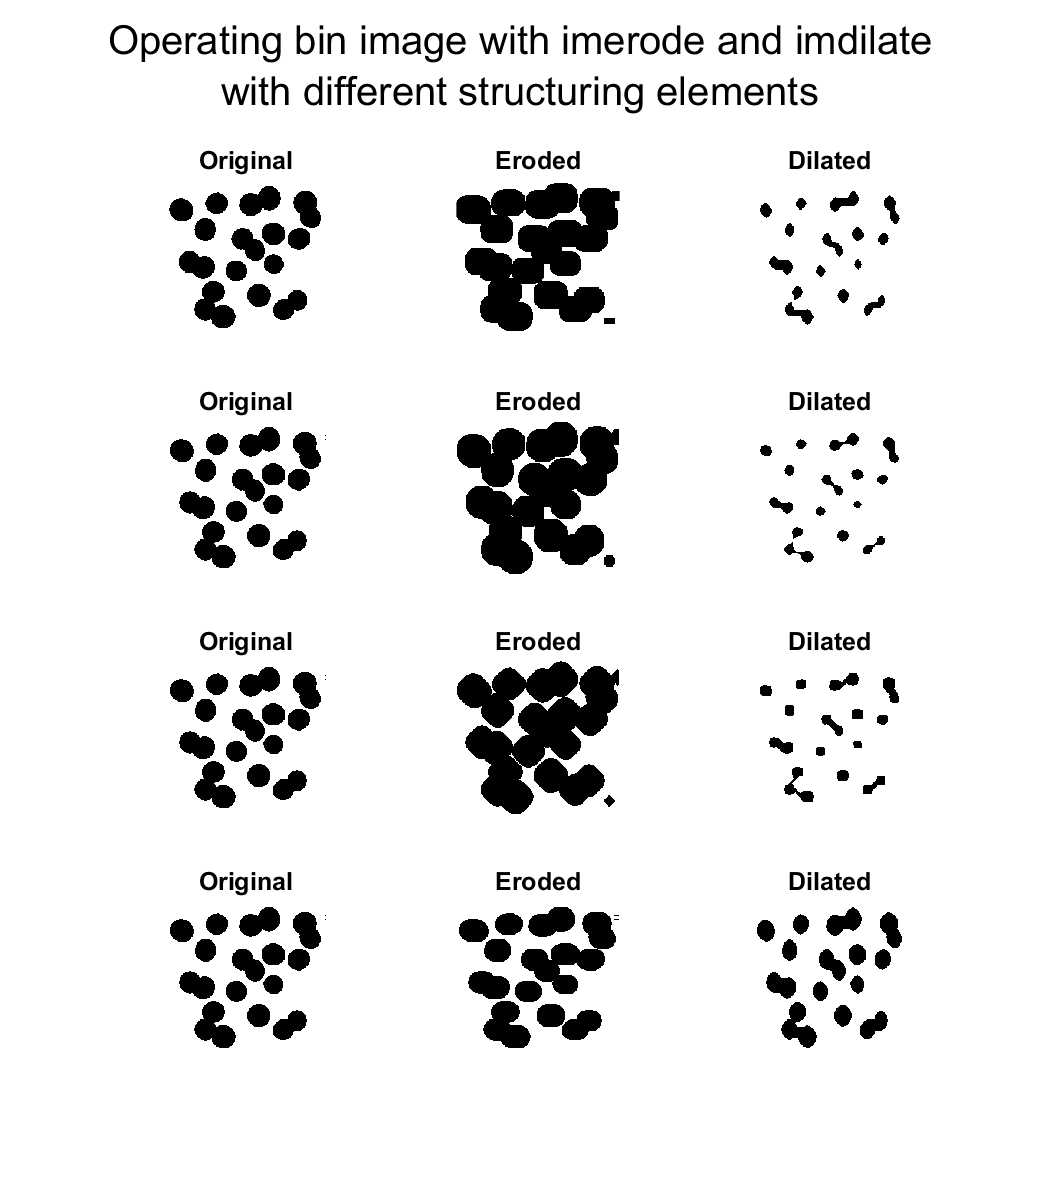
\includegraphics[width=0.75\linewidth]{Doc/Graphics/Part2/part2_Question2.png}
\end{figure}


\newpage
\textbf{Question 3} \textit{Extract internal and external edges of a binary image, and the morphological gradient.}
\begin{figure}[h]
    \centering
    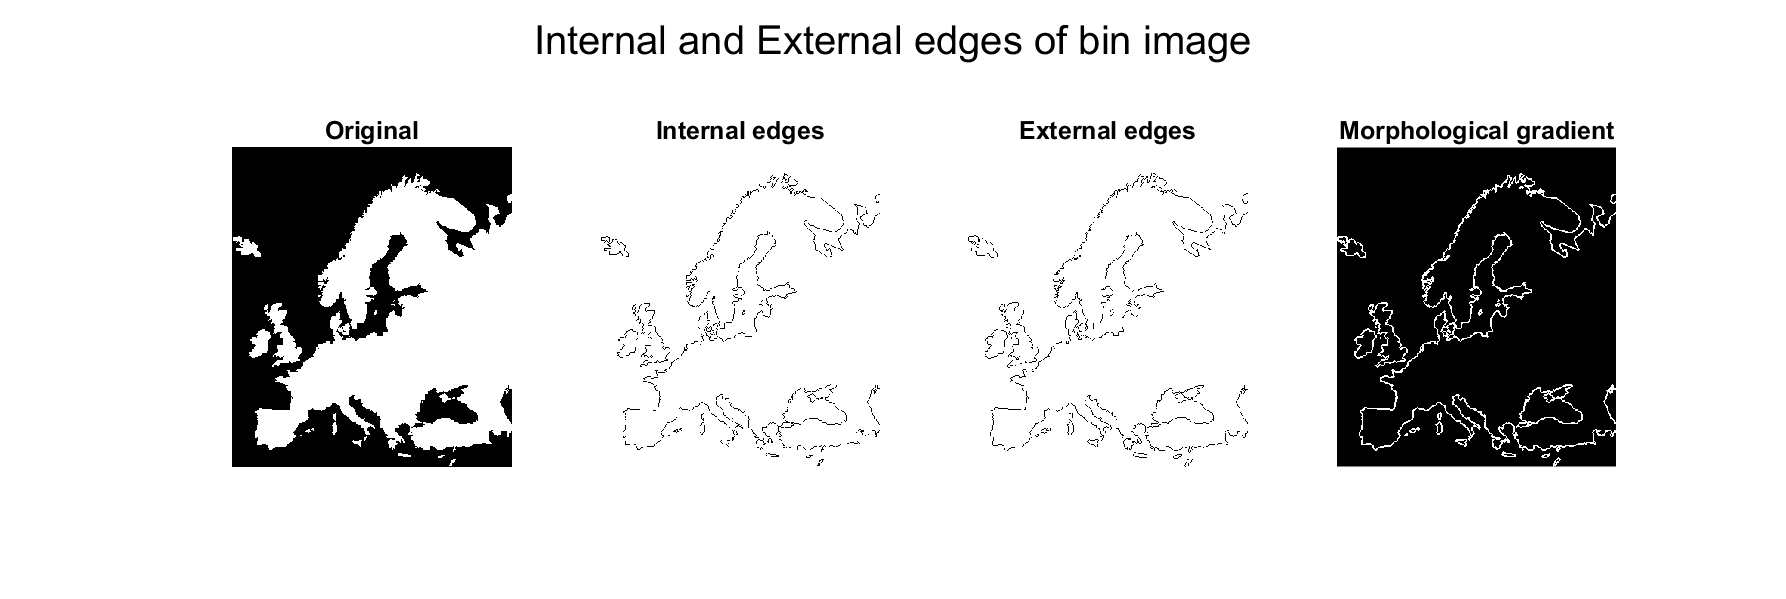
\includegraphics[width=1\linewidth]{Doc/Graphics/Part2/Part2_Question3.png}
\end{figure}


\textbf{Question 4} \textit{As an exercise, write an algorithm that show, in the map of Europe, the distance of each pixel w.r.t. the sea.}
\begin{figure}[h]
    \centering
    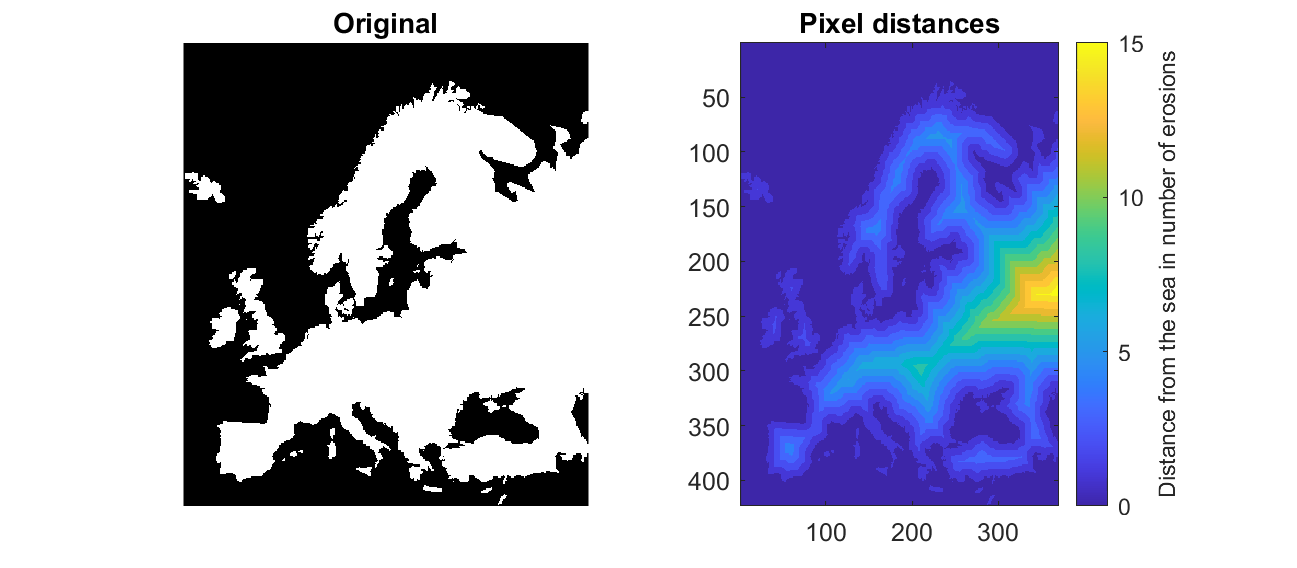
\includegraphics[width=0.75\linewidth]{Doc/Graphics/Part2/part2_Question4.png}
\end{figure}



\textbf{Question 5} \textit{Find an algorithm that detect rectangular objects of ’image2.jpg’.}

\begin{figure}[H]
    \centering
    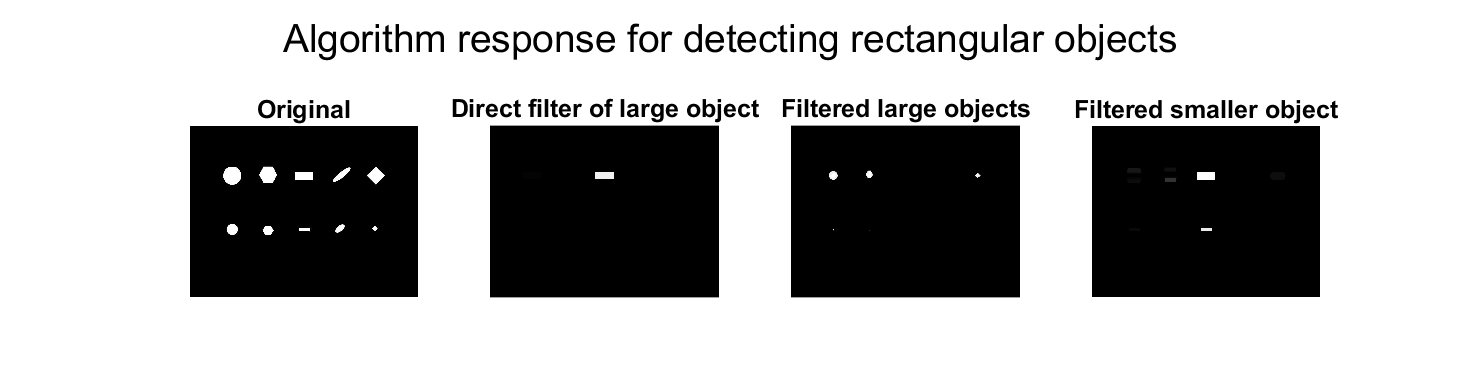
\includegraphics[width=\linewidth]{Doc/Graphics/Part2/Part2_Q5.png}
\end{figure}


\subsection{Morphological Filtering}
\subsubsection{Filters}
\textbf{Question 6} \textit{Define the two morphological filters called opening and closing. What are the effects on a binary image sur as ’image1.jpg’ (use the commands imopen and imclose)?}

\begin{itemize}
    \item \textbf{Opening filter:} is basically erosion followed by dilation. It removes small objects and noise from the foreground and smooths object boundaries.

    \item  \textbf{Closing filter:} is basically dilation followed by erosion. It fills small holes and gaps in the foreground and smooths object boundaries.    
\end{itemize}


The \texttt{imopen()} command seems to reduce some amount of "black-colored noise" from the image and slight sharp inserts in the circle in the bottom left of the original image. The \texttt{imclose()} command seems to remove "white-colored noise" and the outlet of the circle in the top left.

The effects of the commands on \texttt{image1.jpg} can be seen below.

\begin{figure}[H]
    \centering
    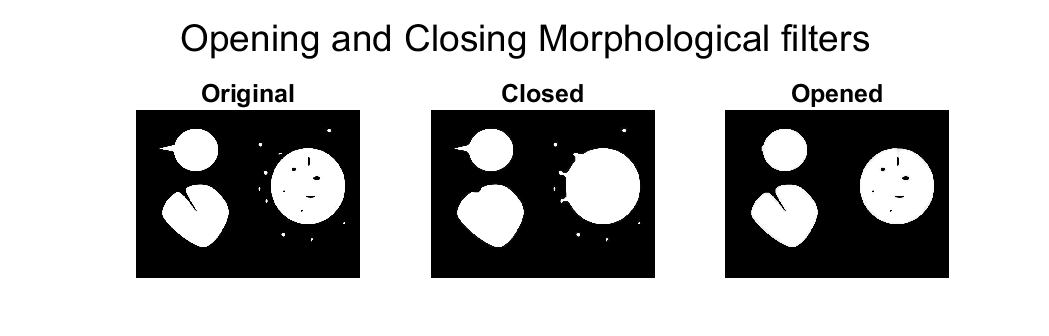
\includegraphics[width=0.75\linewidth]{Doc/Graphics/Part2/part2_Q6.png}
\end{figure}

\subsubsection{Form Detection}
\textbf{Question 7} \textit{The objective being to recognize some forms on images, find a simple algorithm to operate form detection}

See Question 5, can easily be modified for different shapes, i.e. circle, diamond etc.


\textbf{Question 8} \textit{Apply a salt-and-pepper noise: what’s happen with your previous algorithm?}

The algorithm breaks and does not function at all due to the noise in the picture. See below:

\begin{figure}[H]
    \centering
    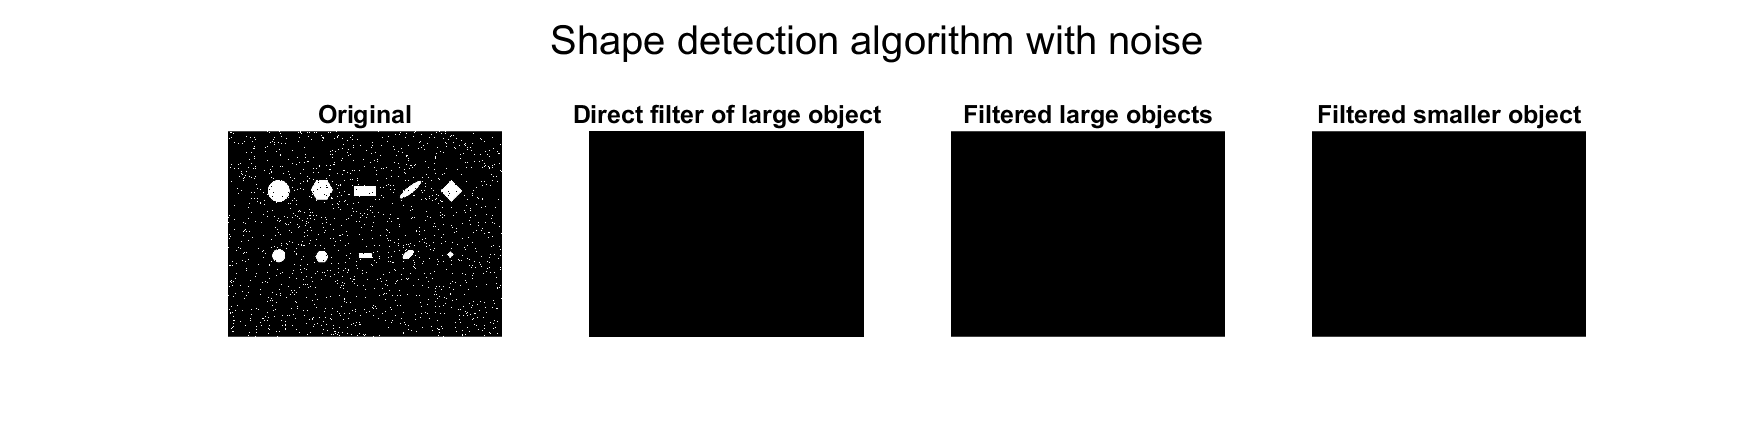
\includegraphics[width=\linewidth]{Doc/Graphics/Part2/part2_Q8.png}
\end{figure}


\subsubsection{Denoising}
\textbf{Question 9} \textit{Use the image Nebuleuse.jpg and apply a salt-and-pepper noise. De-noise the image by filtering.}

\begin{figure}[H]
    \centering
    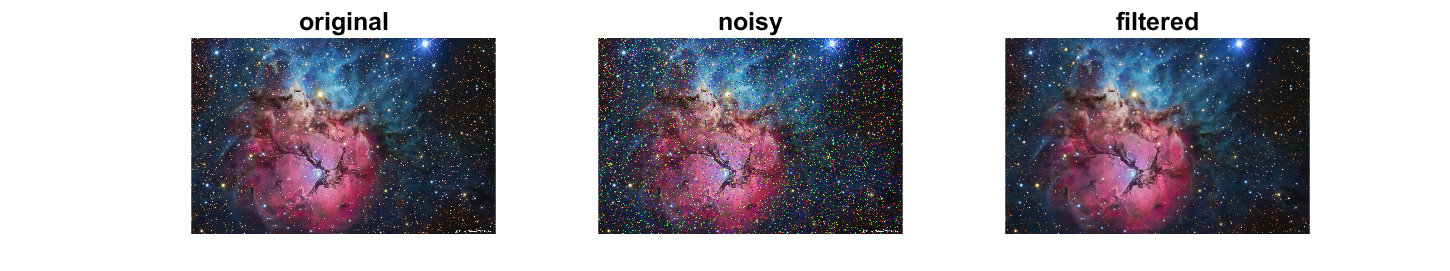
\includegraphics[width=\linewidth]{Doc/Graphics/Part2/part2_Q9.png}
    \caption{Nebula with added and then removed noise}
\end{figure}

\textbf{Question 10} \textit{Apply the same process to the ’Spain Beach’ image to isolate the beach itself.}

\begin{figure}[H]
    \centering
    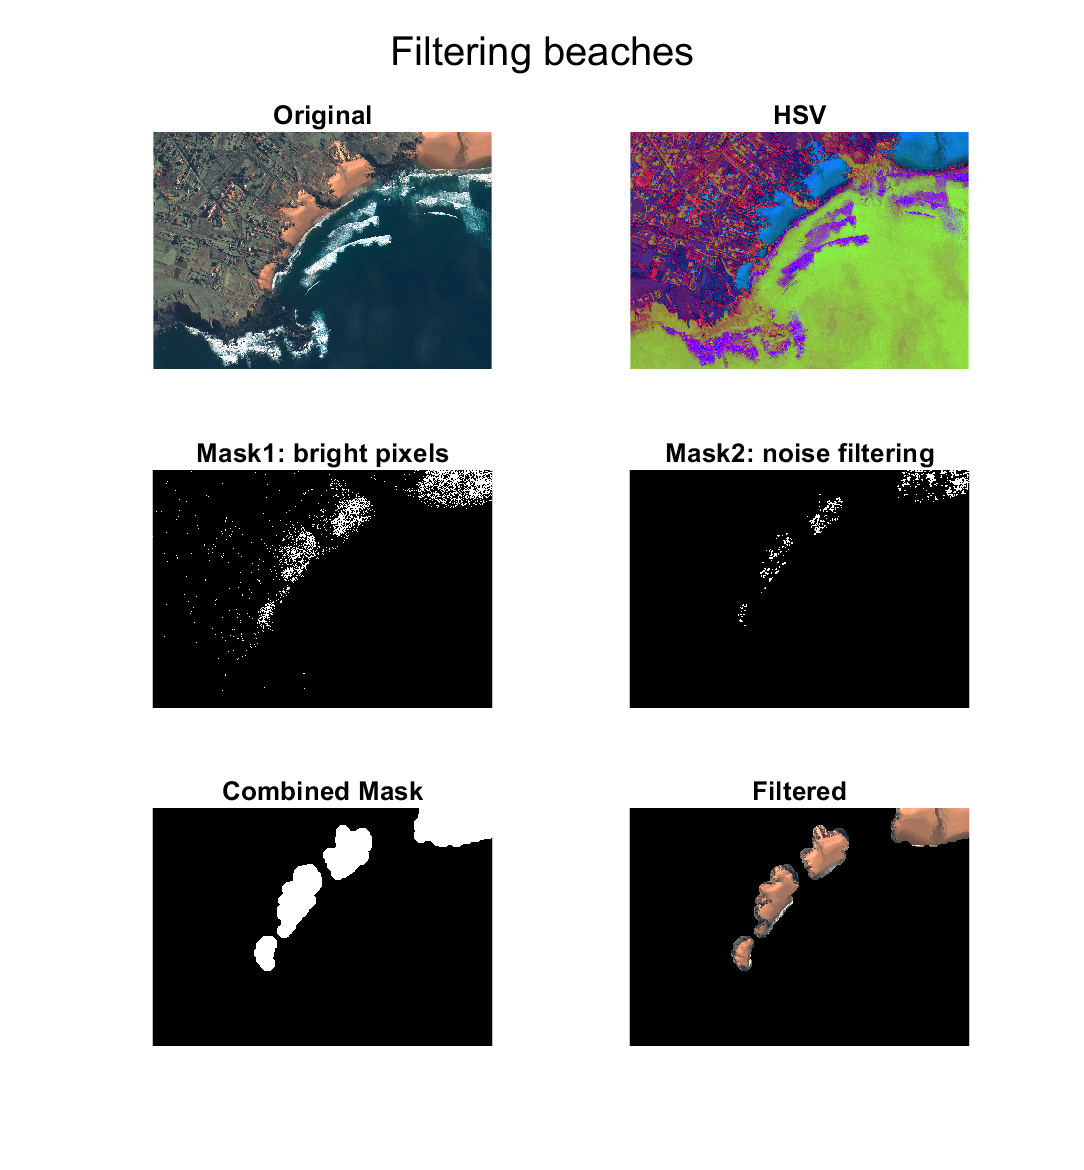
\includegraphics[width=0.5\linewidth]{Doc/Graphics/Part2/part2_Q10.png}
\end{figure}

\subsubsection{Top-Hat \& Black-Hat Filters}
\textbf{Question 11} \textit{Define Top-hat and black-hat process in a 1D function: what is the associated process?}

\begin{itemize}
    \item \textbf{Top-Hat:} This transform is the difference between the original signal and its opening, highlighting small bright features or peaks in the signal.

    \item \textbf{Black-Hat:} This transform is the difference between the closing of the signal and the original signal, highlighting small dark features or valleys.
\end{itemize}


\textbf{Question 12} \textit{Define and operate top-hat and black-hat on a greyscale image. What do you observe?}

\begin{figure}[!ht]
    \centering
    \begin{subfigure}{0.32\textwidth}
        \centering
        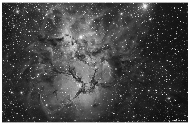
\includegraphics[width=\textwidth]{Doc/Graphics/Part1/Q12_Original_bw.png}
        \caption{Original in grayscale}
    \end{subfigure}
    \hfill
    \begin{subfigure}{0.32\textwidth}
        \centering
        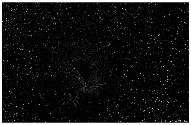
\includegraphics[width=\textwidth]{Doc/Graphics/Part1/Q12_whitehat.png}
        \caption{Top-hat}
    \end{subfigure}
    \hfill
    \begin{subfigure}{0.32\textwidth}
        \centering
        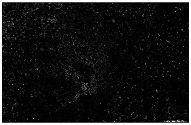
\includegraphics[width=\textwidth]{Doc/Graphics/Part1/Q12_blackhat.png}
        \caption{Black-hat}
    \end{subfigure}
    \caption{Transform results}
    \label{fig:enter-label}
\end{figure}
We can observe that the top-hat transform preserves the small, bright details, while the black-hat transform keeps the dark details, such as the dark gas clouds in the nebula.

% \TODO{What do you observe?? My brain is not working anymore}

% \begin{figure}[H]
%     \centering
%     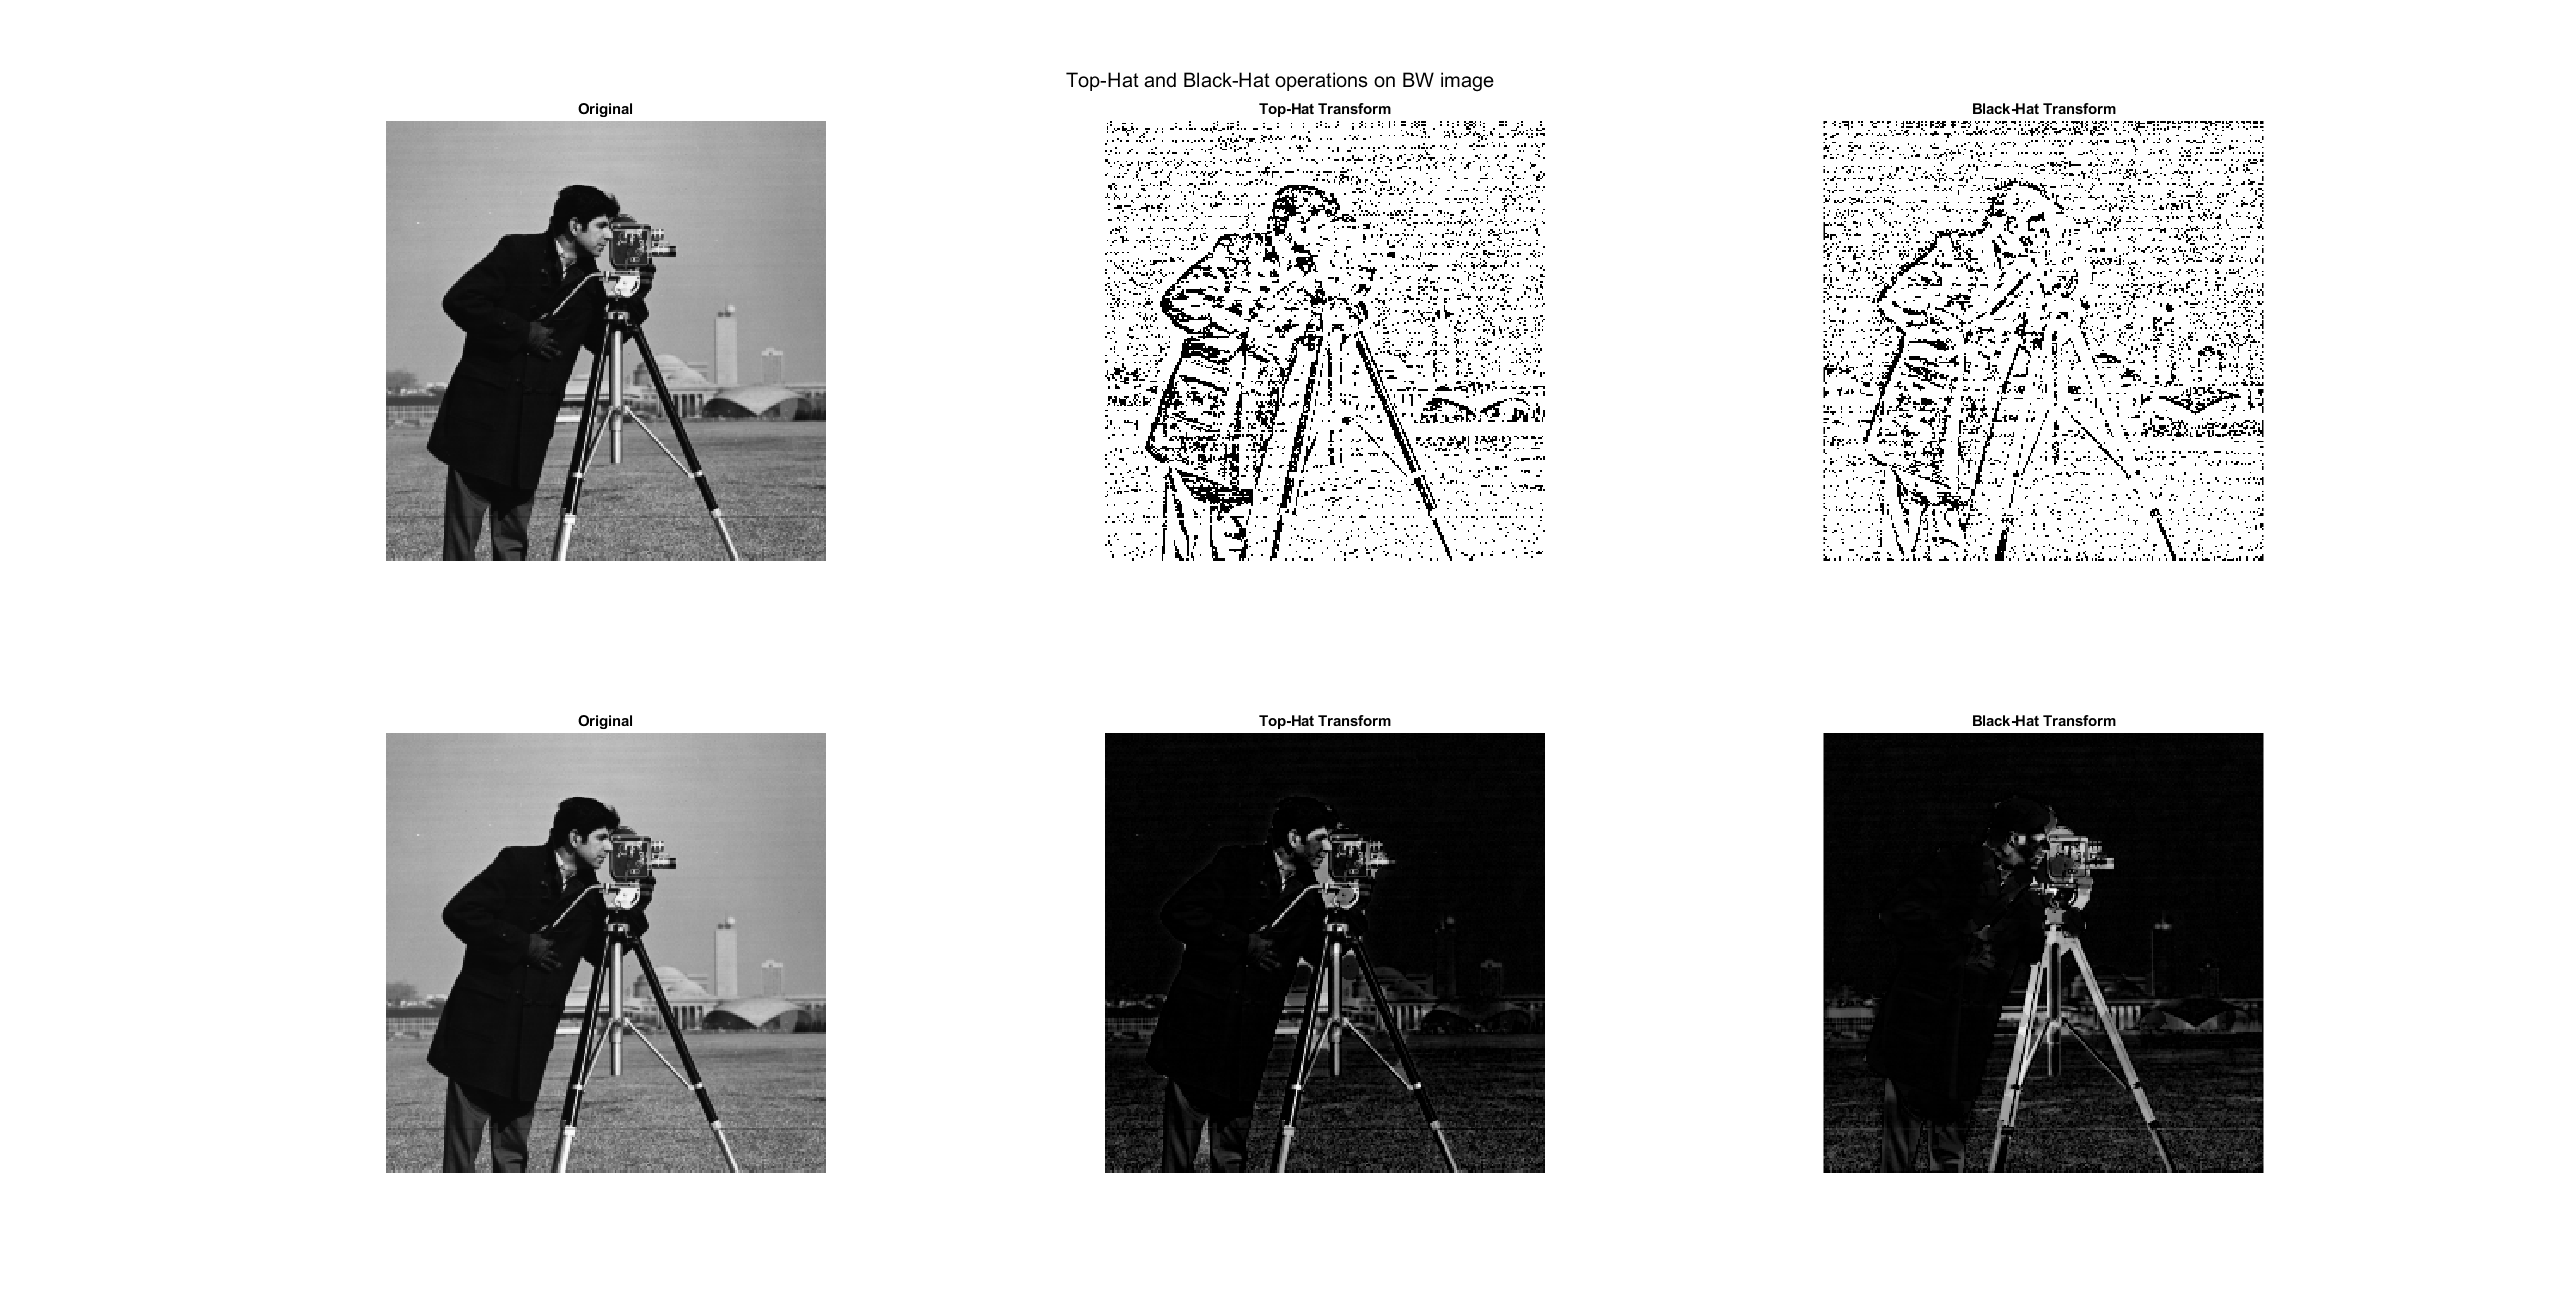
\includegraphics[width=1\linewidth]{Doc/Graphics/Part2/Q12.png}
% \end{figure}
% \FloatBarrier

\newpage
\subsection{Morphological Skeletonization \& Segmentation}
\subsubsection{Skeletonization Process}
\textbf{Question 13} \textit{Write and operate a Skeletonization on the diplodocus.}

\begin{figure}[H]
    \centering
    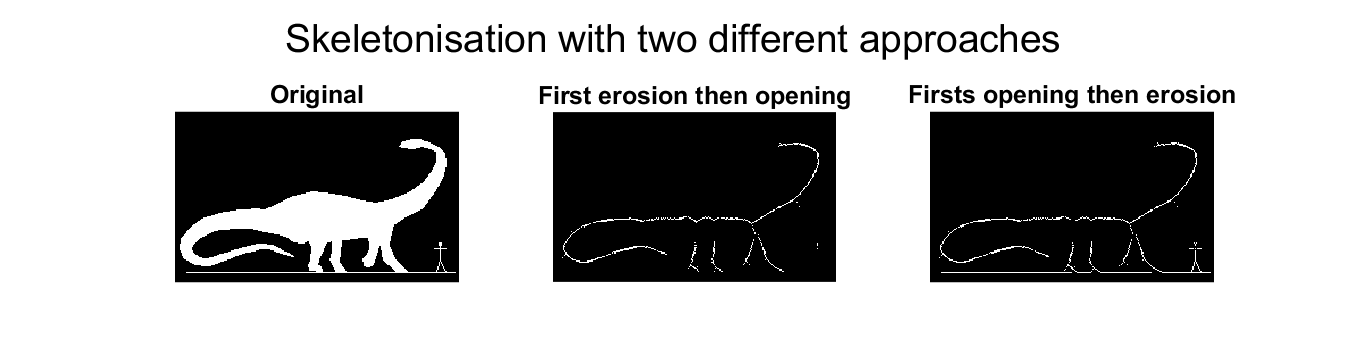
\includegraphics[width=\linewidth]{Doc/Graphics/Part2/part2_Q13.png}
\end{figure}


\textbf{Question 14} \textit{Based on skelittization, find an algorithm that operate a segmentation in a binary image. Apply on ’image1.jpg’.}

\begin{figure}[H]
    \centering
    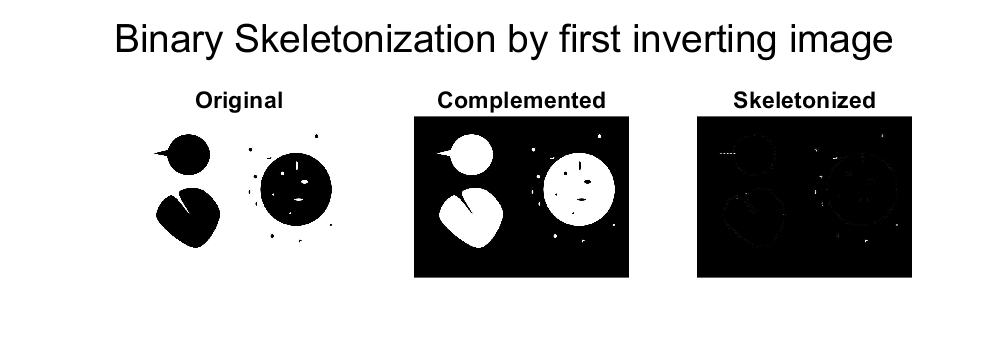
\includegraphics[width=\linewidth]{Doc/Graphics/Part2/part2_Q14.png}
\end{figure}



\newpage
\subsubsection{Image Segmentation}
\textbf{Question 15} \textit{Find a Skeletonization algorithm and operate on the Blood Cells image.}


\begin{figure}[H]
    \centering
    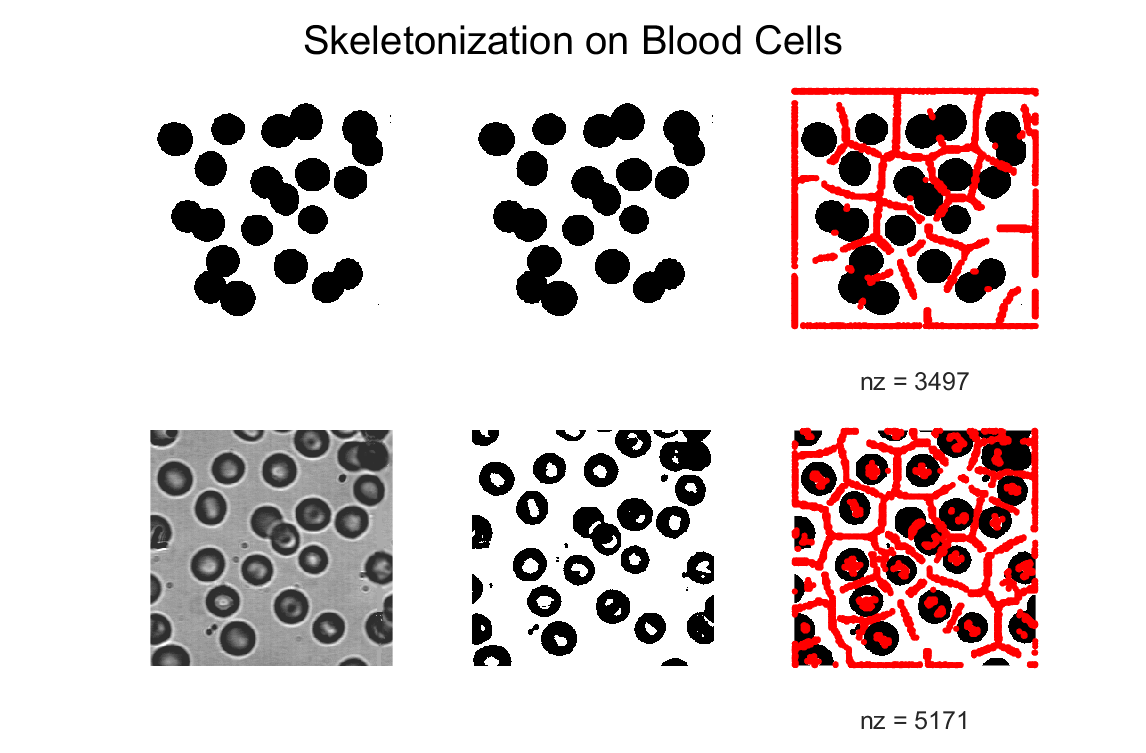
\includegraphics[width=\linewidth]{Doc/Graphics/Part2/part2_Q15.png}
\end{figure}
